\documentclass[russian,]{article}
\usepackage[]{amsmath}
\usepackage{amssymb,amsmath}
\usepackage{ifxetex,ifluatex}
\usepackage{fixltx2e} % provides \textsubscript
\ifnum 0\ifxetex 1\fi\ifluatex 1\fi=0 % if pdftex
  \usepackage[T1, T2A]{fontenc}
  \usepackage[utf8]{inputenc}
\else % if luatex or xelatex
  \ifxetex
    \usepackage{mathspec}
  \else
    \usepackage{fontspec}
  \fi
  \defaultfontfeatures{Ligatures=TeX,Scale=MatchLowercase}
\fi
% use upquote if available, for straight quotes in verbatim environments
\IfFileExists{upquote.sty}{\usepackage{upquote}}{}
% use microtype if available
\IfFileExists{microtype.sty}{%
\usepackage[]{microtype}
\UseMicrotypeSet[protrusion]{basicmath} % disable protrusion for tt fonts
}{}
\PassOptionsToPackage{hyphens}{url} % url is loaded by hyperref
\usepackage[unicode=true]{hyperref}
\hypersetup{
            pdfborder={0 0 0},
            breaklinks=true}
\urlstyle{same}  % don't use monospace font for urls
\ifnum 0\ifxetex 1\fi\ifluatex 1\fi=0 % if pdftex
  \usepackage[shorthands=off,main=russian]{babel}
\else
  \usepackage{polyglossia}
  \setmainlanguage[]{}
\fi
\usepackage{longtable,booktabs}
% Fix footnotes in tables (requires footnote package)
\IfFileExists{footnote.sty}{\usepackage{footnote}\makesavenoteenv{long table}}{}
\usepackage{graphicx,grffile}
\makeatletter
\def\maxwidth{\ifdim\Gin@nat@width>\linewidth\linewidth\else\Gin@nat@width\fi}
\def\maxheight{\ifdim\Gin@nat@height>\textheight\textheight\else\Gin@nat@height\fi}
\makeatother
% Scale images if necessary, so that they will not overflow the page
% margins by default, and it is still possible to overwrite the defaults
% using explicit options in \includegraphics[width, height, ...]{}
\setkeys{Gin}{width=\maxwidth,height=\maxheight,keepaspectratio}
\IfFileExists{parskip.sty}{%
\usepackage{parskip}
}{% else
\setlength{\parindent}{0pt}
\setlength{\parskip}{6pt plus 2pt minus 1pt}
}
\setlength{\emergencystretch}{3em}  % prevent overfull lines
\providecommand{\tightlist}{%
  \setlength{\itemsep}{0pt}\setlength{\parskip}{0pt}}
\setcounter{secnumdepth}{0}
% Redefines (sub)paragraphs to behave more like sections
\ifx\paragraph\undefined\else
\let\oldparagraph\paragraph
\renewcommand{\paragraph}[1]{\oldparagraph{#1}\mbox{}}
\fi
\ifx\subparagraph\undefined\else
\let\oldsubparagraph\subparagraph
\renewcommand{\subparagraph}[1]{\oldsubparagraph{#1}\mbox{}}
\fi

% set default figure placement to htbp
\makeatletter
\def\fps@figure{htbp}
\makeatother

\usepackage[a4paper,left=20mm,right=10mm,top=20mm,bottom=20mm]{geometry}

\usepackage{amsgen, amsmath, amstext, amsbsy, amsopn, amsfonts, amsthm, amssymb, amscd, mathtext, mathtools}
\usepackage{versions}

\usepackage{float}
\restylefloat{table}

\usepackage{xfrac}

\usepackage{hyperref,texlinks}

\usepackage{minted}
\newcommand{\mi}{\mintinline}

% Set line spacing for the whole document
\renewcommand{\baselinestretch}{1}

% RedeclareMathOperator
\makeatletter
\newcommand\RedeclareMathOperator{%
  \@ifstar{\def\rmo@s{m}\rmo@redeclare}{\def\rmo@s{o}\rmo@redeclare}%
}
% this is taken from \renew@command
\newcommand\rmo@redeclare[2]{%
  \begingroup \escapechar\m@ne\xdef\@gtempa{{\string#1}}\endgroup
  \expandafter\@ifundefined\@gtempa
     {\@latex@error{\noexpand#1undefined}\@ehc}%
     \relax
  \expandafter\rmo@declmathop\rmo@s{#1}{#2}}
% This is just \@declmathop without \@ifdefinable
\newcommand\rmo@declmathop[3]{%
  \DeclareRobustCommand{#2}{\qopname\newmcodes@#1{#3}}%
}
\@onlypreamble\RedeclareMathOperator
\makeatother

% Explain
\newcommand{\expl}[2]{\underset{\mathclap{\overset{\uparrow}{#2}}}{#1}}
\newcommand{\explup}[2]{\overset{\mathclap{\underset{\downarrow}{#2}}}{#1}}
\newcommand{\obrace}[2]{\overbrace{#1}^{#2}}
\newcommand{\ubrace}[2]{\underbrace{#1}_{#2}}

% Arrows
\newcommand{\Then}{\Rightarrow}
\newcommand{\Iff}{\Leftrightarrow}
\newcommand{\When}{\Leftarrow}
\newcommand{\Bydef}{\rightleftharpoons}
%\newcommand{\Divby}{\raisebox{-2pt}{\vdots}}
\DeclareRobustCommand{\Divby}{%
  \mathrel{\text{\vbox{\baselineskip.65ex\lineskiplimit0pt\hbox{.}\hbox{.}\hbox{.}}}}%
}

\DeclareMathOperator{\Char}{char}
\DeclareMathOperator{\Ker}{Ker}
\DeclareMathOperator{\Quot}{Quot}
\DeclareMathOperator{\Gal}{Gal}
\DeclareMathOperator{\Aut}{Aut}
\DeclareMathOperator{\id}{id}
\RedeclareMathOperator{\Im}{Im}
\DeclareMathOperator{\ord}{ord}

% Mathbbs
\newcommand{\N}{\mathbb{N}}
\newcommand{\Z}{\mathbb{Z}}
\newcommand{\Zp}{\Z_p}
\newcommand{\Q}{\mathbb{Q}}
\newcommand{\R}{\mathbb{R}}
\renewcommand{\C}{\mathbb{C}}
\newcommand{\F}{\mathbb{F}}

% Short names
\renewcommand{\~}{\sim}
\renewcommand{\phi}{\varphi}
\newcommand{\Have}{\hookrightarrow}
\newcommand{\isom}{\cong}
\renewcommand{\ge}{\geqslant}
\renewcommand{\le}{\leqslant}
\providecommand{\abs}[1]{\lvert#1\rvert}
\renewcommand{\bf}{\textbf}
\renewcommand{\it}{\textit}
\renewcommand{\i}{\item}
\newcommand{\ul}{\itemize}
\renewcommand{\bar}{\overline}
%\newcommand{\ol}{\enumerate}
%\let\ol\enumerate
\newenvironment{ol}{\begin{enumerate}}{\end{enumerate}}
\renewcommand{\b}{\begin}
\newcommand{\e}{\end}
\newcommand{\<}{\langle}
\renewcommand{\>}{\rangle} % Возможно сломает форматирование

\usepackage{pifont}
\newcommand{\cmark}{\ding{51}}
\newcommand{\xmark}{\ding{55}}
\newcommand{\y}{\cmark}
\newcommand{\x}{\xmark}

% Quotes
\usepackage{xspace}
\newcommand{\lgq}{\guillemotleft\nobreak\ignorespaces}
\newcommand{\rgq}{\guillemotright\xspace}

% Consider changing to sfrac
\newcommand{\bigslant}[2]{{\raisebox{.2em}{$#1$}\left/\raisebox{-.2em}{$#2$}\right.}}

\makeatletter
\newenvironment{sqcases}{%
  \matrix@check\sqcases\env@sqcases
}{%
  \endarray\right.%
}
\def\env@sqcases{%
  \let\@ifnextchar\new@ifnextchar
  \left\lbrack
  \def\arraystretch{1.2}%
  \array{@{}l@{\quad}l@{}}%
}
\makeatother

\makeatletter
\newenvironment{nocases}{%
  \matrix@check\sqcases\env@sqcases
}{%
  \endarray\right.%
}
\def\env@nocases{%
  \let\@ifnextchar\new@ifnextchar
  \def\arraystretch{1.2}%
  \array{@{}l@{\quad}l@{}}%
}
\makeatother

% hide LaTeX code from pandoc
\newcommand{\nopandoc}[1]{#1}
\nopandoc{
	\let\Begin\begin
	\let\End\end
}


% Styles for theorems
\usepackage{thmtools}
% renewtheorem
% not works
\makeatletter
\def\renewtheorem#1{%
  \expandafter\let\csname#1\endcsname\relax
  \expandafter\let\csname c@#1\endcsname\relax
  \gdef\renewtheorem@envname{#1}
  \renewtheorem@secpar
}
\def\renewtheorem@secpar{\@ifnextchar[{\renewtheorem@numberedlike}{\renewtheorem@nonumberedlike}}
\def\renewtheorem@numberedlike[#1]#2{\newtheorem{\renewtheorem@envname}[#1]{#2}}
\def\renewtheorem@nonumberedlike#1{  
\def\renewtheorem@caption{#1}
\edef\renewtheorem@nowithin{\noexpand\newtheorem{\renewtheorem@envname}{\renewtheorem@caption}}
\renewtheorem@thirdpar
}
\def\renewtheorem@thirdpar{\@ifnextchar[{\renewtheorem@within}{\renewtheorem@nowithin}}
\def\renewtheorem@within[#1]{\renewtheorem@nowithin[#1]}
\makeatother

\declaretheoremstyle[notefont=\bfseries,notebraces={}{},headpunct={},%
postheadspace={5px},headformat={\makebox[0pt][r]{\NAME\ \NUMBER\ }\setbox0\hbox{\ }\hspace{-\the\wd0}\NOTE}]{problemstyle}
\declaretheorem[style=problemstyle,numbered=no,name=№]{problem}

\declaretheoremstyle[notefont=\bfseries,notebraces={}{},headpunct={ },postheadspace={0px},qed=$\blacktriangleleft$,
headformat={\makebox[0pt][r]{\NAME\ }\setbox0\hbox{\ }\hspace{-\the\wd0}\NOTE},]{solutionstyle}
\declaretheorem[style=solutionstyle,numbered=no,name=$\blacktriangleright$]{solution}
\let\proof\relax
\declaretheorem[style=solutionstyle,numbered=no,name=$\blacktriangleright$]{proof}

\declaretheoremstyle[notefont=\bfseries,notebraces={}{},headpunct={.},postheadspace={4px}]{definitionstyle}
\declaretheorem[style=definitionstyle,numbered=yes,name=Опр]{defn}
\declaretheorem[style=definitionstyle,numbered=no,name=Утв]{stmt}
\declaretheorem[style=definitionstyle,numbered=no,name=Зам]{note}
\declaretheorem[style=definitionstyle,numbered=no,name=Теор]{thm}
\let\lemma\relax
\declaretheorem[style=definitionstyle,numbered=no,name=Лемма]{lemma}

\usepackage{enumitem}
\AddEnumerateCounter{\Asbuk}{\@Asbuk}{\CYRM}
\AddEnumerateCounter{\asbuk}{\@asbuk}{\cyrm}
%\renewcommand{\theenumi}{(\Asbuk{enumi})}
%\renewcommand{\labelenumi}{\Asbuk{enumi})}
\setlist[itemize]{leftmargin=*}
\setlist[enumerate]{leftmargin=*}

\usepackage[at]{easylist}

\def\definemyeasylist#1#2{\expandafter\def\csname el@style@#1\endcsname{\NewList(#2)}}
\def\el{\futurelet\next\domyeasylist}
\def\domyeasylist{\ifx[\next\expandafter\domyeasylistone\else\expandafter\domyeasylistnop\fi}
\def\domyeasylistone[#1]{\begin{easylist}\if\relax\detokenize{#1}\relax\else\csname el@style@#1\endcsname\fi}
\def\domyeasylistnop{\begin{easylist}\NewList}
\def\endel{\end{easylist}}

\definemyeasylist{ul}{Margin1=0cm,Progressive*=1em,
Hang=true,Space=-1pt,Space*=-1pt,Hide=1000,%
Style1*=\textbullet\hskip .5em,%
Style2*=--\hskip .5em,%
Style3*=$\ast$\hskip .5em,%
Style4*=$\cdot$\hskip .5em}

\definemyeasylist{ol}{Hang=true,Mark=.,Space=-1pt,Space*=-1pt,Align=move,
Style2*={(},Mark2={)},Numbers2=l,Hide2=1,%
Numbers3=r,Hide3=2,%
Numbers4=L,Hide4=3}

% Strikeout
\usepackage[normalem]{ulem}
\newcommand{\s}[1]{\ifmmode\text{\sout{\ensuremath{#1}}}\else\sout{#1}\fi}

% Tables
\usepackage{color}
\usepackage{colortbl}
\usepackage{pbox}

\usepackage{tikz}
\usetikzlibrary{chains,shapes,arrows,positioning}



\usepackage[]{algorithm2e}

\usepackage{subfig}

\declaretheoremstyle[%
spaceabove=-6pt,%
spacebelow=6pt,%
headfont=\normalfont\itshape,%
postheadspace=1em,%
qed=\qedsymbol%
]{mystyle} 
\declaretheorem[name={Доказательство},style=mystyle,unnumbered,
]{Proof}

\usepackage{tikz}
\newcommand*\circled[1]{\tikz[baseline=(char.base)]{
		\node[shape=circle,draw,inner sep=1pt] (char) {#1};}}
	
\newtheorem{theorem}{Теорема}

\renewcommand{\G}{\mathcal{G}}

% \excludeversion{proofstar}
\includeversion{proofstar}
\excludeversion{proofstardetailed}

\title{Алгоритм Бермана-Карпински приближённого решения задачи \mbox{(1, 2)-TSP} с точностью $\frac{8}{7}$}
\date{}
\author{}
\begin{document}
\maketitle
\bibliographystyle{unsrt}
%\bibliographystyle{gost780s}

\section{Введение}
Пусть дан полный граф $K_n = (V, E)$ с весами рёбер $c \in \R^E$. \textit{Задача коммивояжёра} (TSP) заключается в том, чтобы найти гамильтонов цикл (обход) в G минимальной стоимости. Если $c_{ij} = c_{ji}\ \forall (i, j)  \in E$, говорят, что задача симметрична. 

Если веса рёбер удовлетворяют неравенству треугольника, говорят о метрической задаче коммивояжёра. Метрическая задача коммивояжёра --- одна из старейших известных NP-полных задач (доказательство NP-полноты см. в \cite{JP85}). Наилучший известный сейчас результат --- приближение с точностью $\frac{3}{2}$\cite{C76}. 

Внимания заслуживает случай симметричной задачи коммивояжёра с весами 1 и 2, называемый (1,2)-TSP. Поскольку $\forall a, b, c \in \{1, 2\} \ a\le b+c$, неравенство треугольника всегда выполняется, и это --- подкласс метрической задачи коммивояжёра. (1, 2)-TSP можно рассматривать как обобщение задачи о гамильтоновом пути, требующее наличия в гамильтоновом пути как можно меньшего количества рёбер веса 2.

Было доказано (\cite{EK01}), что нельзя построить приближение лучше $\frac{741}{740}$. Наилучший известный алгоритм Пападимитриу-Яннакакиса \cite{PY93} предоставлял приближение $7/6$ и был незначительно улучшен до $65/56$ \cite{BR05}. 

Берман и Карпински в своей статье \cite{BK06} привели новую методику, позволившую улучшить точность приближения до $\frac{8}{7}$. Этот алгоритм мы и рассмотрим. Поскольку статья очень объёмная, а проект практический, некоторые выкладки будут пропущены, а некоторые утверждения оставлены без доказательства.

\subsection{\NP-полнота}
Поставим задачу формально.

TSP $= \{ (G, \mathbf{w}, k): \exists$ цикл во взвешенном графе $(G, \mathbf{w})$, посещающий каждую вершину ровно 1 раз и имеющий вес $\le k \}$

\begin{theorem}
	TSP --- \NP-полно.
\end{theorem}
\begin{Proof}
 $ $
 
 \begin{itemize}
  \i TSP $\in \NP$\cite{BA09}:
 
  Сертификатом является собственно обход. За полиномиальное время проверяется, что такой обход в графе действительно существует, и что его длина $\le k$.
 
  \i UHAMPATH $\le_p$ TSP: \cite{M17}
 
  Сопоставим всем рёбрам единичные веса и возьмём $k = n$. Путь длины $n$, проходящий через все вершины, обязан быть гамильтоновым. \qedhere
 \end{itemize}
\end{Proof}

\subsection{Эквивалентная формулировка}
Представим экземпляр задачи (1,2)-TSP как граф $G$, вершины которого --- точки метрики, а рёбра --- пары вершин на расстоянии 1. Пусть в $G$ $n$ вершин, и можно найти его покрытие $k$ путями (простыми и вершинно непересекающимися). Тогда эти пути содержат $n-k$ рёбер и их можно соединить в обход, где ребро из конца одного пути в начало другого будет иметь вес 2. Стоимость обхода будет $n+k$, задача --- минимизировать $k$. Если оптимальное решение содержит $n+k^*$ рёбер, нам нужно найти покрытие путями из $\le \frac{1}{7}n+\frac{8}{7}k^*$ путей. Будем далее решать такую задачу.

\section{Алгоритм малых улучшений}
Будем поддерживать текущее решение алгоритма как множество рёбер $A$ ("algorithm"), являющееся 2-паросочетанием (то есть, у вершины может быть не более двух инцидентных ей рёбер из $A$). Пусть в нём $k_A$ путей и циклов, $m_A$ вершин в циклах, $s_A$ синглтонов (т. е. компонент связности размера 1). Это решение можно преобразовать с помощью множества рёбер $C$ ("change") в новое решение $A \oplus C$. 

$C$ улучшает $A$, если 
\begin{enumerate}[label=\protect\circled{{\arabic*}}]
	\i $A \oplus C$ --- 2-паросочетание;
	\i $k_{A \oplus C} < k_A$ или
	\i $k_{A \oplus C} = k_A$ и $m_{A \oplus C} > m_A$, или
	\i $k_{A \oplus C} = k_A$ и $m_{A \oplus C} = m_A$ и $s_{A \oplus C} < s_A$
\end{enumerate}

Алгоритм K-IMPROV:

\begin{algorithm}[H]
 A = $\emptyset$\;
 \While{$\exists C, |C|<K, C$ улучшает $A$}{
  $A \gets A \oplus C$\;
 }
\end{algorithm}

Предположим, что для некоторой константы $K$ выполняется 
$$(*) \text{ либо } k_A \le \frac{1}{7}n+\frac{8}{7}k^*, \text{ либо } \exists C: C \text{ улучшает } A \textbf{ и } |C|\le K.$$
Заметим, что
\begin{itemize}
 \i нельзя провести более чем $n$ улучшений вида \circled{2}, т. к. число путей и циклов получится $\le 0$;
 \i нельзя провести более чем $n$ улучшений вида \circled{3} подряд без улучшения вида \circled{2}, т. к. в циклах получится $>n$ вершин;
 \i нельзя провести более чем $n$ улучшений вида \circled{4} подряд, т. к. иначе будет $< 0$ изолированных вершин. 
\end{itemize}
То есть, можно провести не более чем $n^3$ улучшений.

Проверка всех пунктов \circled{1} --- \circled{4} занимает $O(n)$.

Перебор всех допустимых вариантов $C$ в самой простой реализации (перебор всех подмножеств множества рёбер) занимает $O((n^2)^K)$. Авторы статьи утверждают, что время работы поиска улучшения можно сократить до  $O(n^K)$, но далее (в разделе про тестирование) описывается, почему это в нашем случае не так важно. Окончательно, время работы K-IMPROV составляет $O(n^{K+4})$.

\subsection{Доказательство утверждения (*)}
В статье \cite{BK06} утверждение доказывается для $K=21$, в расширенной версии статьи --- для $K=15$.
\begin{proofstar}
Зафиксируем оптимальное решение, 2-паросочетание $B$ ("best"), т. ч. $k_B = k^*$. Пусть $D$ --- множество рёбер, оба конца которых лежат в одном и том же цикле $A$. Пусть $\G$, \textit{вспомогательный граф (auxilary graph)}, --- граф, содержащий вершины графа $G$ и рёбра $(A \cup B) \setminus D$. Покрасим его рёбра в три цвета.
Белые из $A \setminus B \setminus D$, чёрные из $B \setminus A \setminus D$ и серые из $(A \cap B) \setminus D$. 

\begin{defn} 
\textit{Чередующийся путь (alternating path)} (ЧП) ---  путь, начинающийся и заканчивающийся чёрными рёбрами, в котором чёрные и белые рёбра чередуются.
\end{defn}

\begin{defn}
\textit{A-объектами} назовём пути и циклы $A$ . Для A-объекта определим \textit{начальную вершину (initial node)} как вершину, которая может быть первой или последней вершиной ЧП и при этом принадлежит A-объекту. 
\begin{itemize}
\i Для A-пути начальные вершины --- его концы. 
\i Для A-цикла $C$ возьмём за начальные вершины такие две, что в $C$ существует гамильтонов путь из одной в другую, который может быть продолжен двумя чёрными рёбрами до двух других вершин. То, что они всегда существуют в цикле из $\le 7$ вершин, доказано далее.
\end{itemize}
\end{defn}

\begin{defn} 
\textit{Фишка (или монетка)} --- абстрактная делимая единица, которая распределяется по вершинам. Изначальное распределение фишек задаётся весами вершин. Общее количество фишек --- сумма этих весов.
\end{defn}

Если $B$ состоит из $k^*$ путей, оптимум имеет стоимость $n+k^*$ и множество A даёт достаточное приближение, если оно имеет стоимость $\le \frac{8}{7}(n+k^*)$, т. е. если оно состоит из $\le \frac{1}{7} + \frac{8}{7}k^*$ A-объектов. Возьмём $n+8k^*$ фишек и докажем, что для того, чтобы A было достаточно хорошим приближением, каждый A-объект должен содержать 8 фишек.
Заметим: вершина, инцидентная $2-a$ вершинам B, содержит $1+4а$ фишек (сумма их всех $2k^*$). 

Изначально фишки пути есть фишки его концов и фишки цикла есть фишки всех его вершин. Оставшиеся фишки содержатся в чередующихся путях. За каждую свою вершину, которая ещё не находится в каком-то A-объекте, ЧП забирает $0.5$ фишки. Оставшиеся $0.5$ фишек могут быть собраны либо другим ЧП, в который входит эта вершина, либо распределены по каким-то другим правилам (см. далее). ЧП будет отдавать свои фишки тем A-объектам, которые содержат его начальные вершины. Если разбить ЧП на два, каждый из них будет содержать только одну начальную вершину, и поэтому давать свои фишки только одному A-объекту.

Обычно А-путь содержит два конца, и каждый из них --- начальная вершина ЧП, который даёт этому пути $2 \frac{1}{2}$ фишек. Цикл обычно содержит $4+a$ вершин и содержит 2 начальных вершины ЧП, которые дают циклу $\frac{3-a}{2}$ фишек.

Могут быть отклонения от обычного случая. Если А-объект содержит менее 2-х начальных вершин, он собирает больше фишек с вершин, которые он содержит. Если А-объект --- синглтон, то каждая начальная вершина даёт ему 3 фишки. Если цикл содержит более 6 вершин, в нём не будет начальных вершин. Вершина, инцидентная только одному ребру из $B$, имеет 4 дополнительных фишки, и мы будем опускать особые случаи, вызванные такими вершинами.

\subsection{Очень маленькие улучшения}
В некоторых случаях возможны улучшения, добавляющие только одно ребро. Обсудим их, а дальше будем предполагать, что они не встречаются.

\begin{itemize}
\i Чёрное ребро $e$, соединяющее две начальные вершины. Если оно соединяет два разных А-объекта, они сливаются в один. Если сливаемый объект --- цикл, приходится удалить одно из его рёбер. Если $e$ содержит начальные вершины одного А-объекта, это обязан быть А-путь, и вставка ребра превращает этот путь в цикл.
\i Ребро, соединяющее А-синглтон с другим А-объектом (за исключением случая, когда синглтон соединяется со средней вершиной А-пути из трёх вершин --- иначе улучшение типа \circled{4}).
\end{itemize}

Предположим, что нет очень маленького улучшения, и есть ЧП $R$, начинающийся в $u$, а $\{u\}$ --- А-синглтон. Тогда для пути (v, w, x) и некоторого $y$ путь $R$ начинается с $(u, w, v, y)$. Когда мы считаем $R$ возможной частью улучшения, мы берём "сокращённую" версию $R$, начинающуюся с $(v, y)$. Так как мы предположили, что вставка одного ребра не приведёт к улучшению, это законно. С одной стороны, мы забываем, что $R$ начинается с синглтона и поэтому должен собрать лишнюю $\frac{1}{2}$ фишки. С другой стороны, мы забудем, что $R$ собирает $\frac{1}{2}$ фишки на вершине $w$.

\subsection{Начальные вершины циклов}
\begin{stmt}
Пусть $C$ --- цикл A с $\le 7$ вершинами с $|C|$ фишками (т. е. у него все вершины смежны с двумя рёбрами из $B$).

Пусть $\hat{C}$ --- множество вершин из $C$, и $\hat{K} \subset \hat{C}$ --- множество вершин, инцидентных двум чёрным вершинам. 

Покажем, что какие-то две вершины из $\hat{K}$ согласованы в том смысле, что они --- концы гамильтонова пути в $\hat{C}$.
\end{stmt}
\begin{proof}$ $\\
\begin{itemize}
\i Если $|\hat{K}| = 2$, то $\hat{K}$ --- согласованная пара, потому что множество рёбер $B$, содержащихся в $C$, образует единственный путь.

\i Пусть $|\hat{K}| \ge 3$. 

Предположим, что две вершины $\hat{K}$, $u$ и $v$, соседние на цикле $C$. Тогда они согласованы, т. к. мы можем сделать путь, удалив ребро $(u, v)$ из $C$.

Иначе они не смежны, и получаем, что $|\hat{K}| \le |\hat{C}|/2$. Это означает, что $|\hat{K}| = 3$ и $|\hat{C}| = 6$.

Т. к. $\hat{K}$ содержит 3 вершины, $B$ покрывает $\hat{C}$ двумя путями. Один из этих путей содержит 1 вершину и 0 рёбер, другой 5 вершин и 4 ребра. Следовательно, 2 ребра $B$ содержатся в $\hat{C} \setminus \hat{K}$. БОО, $C$ --- цикл $(u_0, \dots, u_5)$, $\hat{K} = \{u_0, u_2, u_4\}$ и $\{u_1, u_3\} ]in B$. Тогда мы можем обойти $\hat{C}$ так: $(u_0, u_5, u_4, u_3, u_1, u_2)$. \qedhere
\end{itemize}
\end{proof}

\subsection{ЧП с дефицитом --- общий метод}
Пусть $R$ --- ЧП. По нашим правилам, он собирает $\frac{1}{2}$ фишек за каждую свою вершину, за исключением концов путей и вершин циклов. Мы не собираем больше потому, что каждая из таких вершин может принадлежать более чем одному ЧП.

Есть несколько методов дать $R$ больше фишек:
\begin{itemize}
\i Распределить фишки серых вершин.
\i Разбить ЧП $P$, проходящий через цикл, созданный $R$. Рассмотрим одну из образовавшихся половинок, $P$.
\begin{itemize} 
\i Если она короткая, можно слить цикл с A-объектом, содержащим начальную точку $P$. 
\i Если она длинная, ей не надо собирать фишки с её рёбер в цикле, и эти фишки можно передать $R$.
\end{itemize}
\end{itemize}

\subsection{Избегаем плохих случаев}
\subsubsection{S-дуги --- Избегаем их или находим им дополнительные фишки}

\begin{defn}
\textit{Дуги (arcs)} --- чёрные рёбра, содержащиеся в путях.
\end{defn}

Дуги потенциально проблематичны, так как могут позволить короткому ЧП создать больше циклов, так как они позволяют получить цикл из одного фрагмента A-пути и одного чёрного ребра (собственно, дуги). В этом случае, в ЧП перед этой дугой и после неё идут белые рёбра (или конец пути). 
\begin{defn}
Назовём такую конструкцию \textit{S-дугой} (short cycle making arc). Число вершин на фрагменте пути, соединяющем концы дуги, назовём \textit{длиной дуги}.
\end{defn}

Избежим создания S-дуг декомпозицией чёрных и белых рёбер в множество ЧП. Когда сделать это будет невозможно, мы наделим такие S-дуги серыми вершинами, что даст им дополнительные фишки. 

Чтобы применить эту технику, рассмотрим \textit{цепь} дуг $Q$ ---  путь, образованный дугами, содержащимися в А-пути $P$. Для общности продлим $P$ в оба направления одним \textit{фиктивным белым ребром}. Будем принимать решение, как соединить элементы цепи со смежными белыми рёбрами, когда будем строить ЧП. Соединение дуги с фиктивным белым ребром неявно делает её начальной вершиной её ЧП.

\begin{note}
Решения о разбиении внутри цепи могут быть неоднозначными, и зависят от того, как мы захотим сделать.
\end{note}

Как разрешать неоднозначности?

Сначала возьмём дугу $a_0 \in Q$ с наименьшим приоритетом. Далее, удостоверимся, что никакая другая дуга в $Q$ не является S-дугой. Стартуя из любого конца $Q$, двигаемся к $a$. На этом конце $Q$ поступаем произвольно. По индукции рассмотрим другой конец дуги $a \ne a_0$. На другом его конце мы приняли произвольное решение. Если это решение соединило $a$ с белым ребром, направленным от него, соединим $a$ с белым ребром, направленным к нему, иначе поступим произвольно.

\begin{proofstardetailed}
Хороший случай 1.
Дуга a в цепи $Q$ \textit{прямо достижима} из конца A-пути, т. е. вершина внутри дуги $a$ соединена чёрным ребром с этим концом. Дадим $a$ наименьший приоритет и не получим при этом неблагоприятных последствий. Если мы хотим создать улучшение, используя ЧП, содержащий S-дугу $a$, мы увеличим количество объектов, создав цикл, но уменьшим его обратно, вставив ребро, которое соединяло дугу с концом пути, и уберём смежное ему из цикла.

Хороший случай 2.
Конец $Q$, смежный его первой дуге $a$, смежен к белому ребру $b$, направленному в $a$. Мы можем оставить $a$ с минимальным приоритетом, и финальное решение, соединяющее $a$ с $b$, будет гарантировать, что это не S-дуга.

Хороший случай 3. 
Вершина $u$ смежна двум дугам $Q$ и двум рёбрам, расположенным как на рис. 4. Мы можем дать $a_0$ минимальный приоритет, и решение в $u$ будет соединять $a_0$ с $e_0$ и $a_1$ с $e_1$, что будет гарантировать, что это никогда не станет S-дугой.

Хороший случай 4.
$Q$ состоит из лишь одной дуги $a$ длины 4, и $a$ становится S-дугой, т. е. $a$ смежна двум серым рёбрам, которые внутри неё (рис. 5). Есть 2 ЧП, один с последовательностью рёбер $\{b_0, e_0, a, e_2, b_3\}$, другой с $\{b_1, e_1, b_2\}$. Поменяем соединения так, чтобы были последовательности $\{b_0, e_0, a, g_1, b_2\}$ и $\{b_1, g_0, a, e_2, b_2\}$, и каждый из этих двух ЧП сможет получить $2\frac{1}{2}$ фишек.

Хороший случай 5. $Q$ содержит две последовательные дуги, различающиеся в длине ровно на 2 (рис. 6). Мы можем дать $b_0$ наименьший приоритет, потому что ситуация почти такая же, как в прямом попадании. В частности, в ЧП можно заменить последовательность рёбер $e_0, b_0, e_1$ "обходным путём" $e_0, b_1, e_2$. 

Следовательно, если $Q$ состоит толььо из одной дуги $a$ и мы делаем её S-дугой, длина $a$ по крайней мере 5, и она смежна двум серым рёбрам внутри себя.

Хороший случай 6.
$Q$ содержит две подряд идущие дуги, $b_0$ и $b_1$, где $b_1$ смежно концу пути $P$ и $b_0$ --- нет (представим, что на рис. 6 ребро $e_2$ есть первое ребро $P$). Тогда мы можем дать наименьший приоритет $b_0$, потому что $b_1$ даёт прямое попадание в $b_0$ в случае, если последний станет S-дугой.

Хороший случай 7.
$Q$ содержит дугу $b$, смежную концу $P$ (рис. 7). Если у нас не случай 2, то ребро $g$ серое, и ребро $e_0$ белое. Будем делать похоже на пункт 4. У нас сесть два ЧП, один начинается с $b, e_0, b_0$, другой имеет фрагмент $b_1, e_1, b_2$. Заменим их, соединив $b$ с $b_1$ вместо $b_0$, последовательность $b, g, b_1$, и соединив $b_0$ с $b_2$, последовательность $b_0, e_0, b, e_1, b_2$. Оба этих новых ЧП используют ребро $b$, но первое удаляет $g$ из $P$ и собирает 1 фишку, и второе удаляет $e_0$ и $e_1$, собирая 2 фишки. 
\end{proofstardetailed}

Далее авторы статьи рассматривают 7 "хороших случаев" для цепей. Это очень громоздко, поэтому здесь это приводиться не будет.

\begin{defn}
Цепи, которые не подпадают ни под один из этих случаев, назовём \textit{проблемными}. Они могут образовать \textit{суперцепь} из цепей, соединённых серыми рёбрами. Если такая цепь содержит конец $P$, назовём её \textit{терминальной}. 
\end{defn}

Из разбора хороших случаев и определения "плохой" цепи следует, что:
\begin{enumerate}
\i Проблемная терминальная цепь не может быть соединена в суперцепь с не-проблемными.
\i Терминальная проблемная цепь состоит только из рёбер, смежных своему концу.
% (обозначим его $u$), потому что мы не можем применить методы случаев 3 и 6, и поскольку 2 и 7 неприменимы, и поскольку другой конец/концы этой дуги /дуг смежны паре серых вершин. Поэтому если эта цепь состоит из одной дуги, ЧП, начинающийся в этом ребре, соберёт $2\frac{1}{2}$ фишек с 3-х серых вершин, и эта дуга имеет длину $\ge 5$. Если цепь состоит из двух дуг, она может собрать фишки с 4-х серых рёбер, и более длинная дуга имеет длину $\ge 7$, ЧП, начинающийся из более длинной дуги, наберёт 4 фишки.

\i Как забрать у терминальной проблемной цепи фишки?
\begin{itemize}
\i Если нетерминальная проблемная цепь имеет только одну дугу, то это дуга длины 5 или более, и она смежна двум серым рёбрам, направленным внутрь. Мы можем взять дополнительную фишку у любого из этих рёбер.
\i Нетерминальная проблемная цепь с более чем одной дугой смежна с двумя серыми рёбрами на своих концах. Решим, что соберём фишку с одного из этих рёбер. Дадим наименьший приоритет дуге длины $\ge 6$, которая содержит внутри себя серое ребро. %Скажем, что дуга, смежная этому серому ребру, первая. Если первая дуга имеет длину $\ge 6$, мы даём ей наименьший приоритет. Если она длины $< 6$, идём по цепи, покане увидим увеличение длины более чем на 1, или от 5 до 6. Заметим, что после увеличении длины цепи на 1 мы не можем закончить цепь, а после увеличения длины на 2 можно применить метод из Случая 5, и поэтому после первого большого увеличения мы будем иметь длину $\ge 3+3=6$.
\end{itemize}
\end{enumerate}

%Идя по цепи, мы посещаем вершины (начиная с двух вершин начального серого ребра), и мы не можем вернуться в уже посещённую вершину, потому что чёрные и серые рёбра не могут образовывать короткий цикл. Если мы увеличим длину дуги на 1, мы увеличим дипапазон посещённых вершин не вводя новую дырку, и если мы уменьшим длину дуги, мы заполним дырку. Если начнём в дуги длины 3, у нас нет дырки, и мы не можем уменьшить длину дуги до первого большого увеличения. Если мы начнём с дуги длины 4, будет одна дырка,и мы можем уменьшить длину дуги один раз, но это не может быть концом дуги, и начать с уменьшения мы тоже не можем (это будет дуга длины 2, а это не является дугой), поэтому если мы избегаем длины 6, то у нас будет последовательность длин 4, 5, 4, а далее только увеличения. Если начнём с длины 5, первое уменьшение не может быть 1, потому что оно закрывает чёрный/серый цикл, длины 2, т. к. это случай 5, и 3, т. к. дуг длины 2 нет, поэтому это может быть только увеличение.

\subsubsection{Избегаем терминальных коротких циклов}
\begin{stmt}
Пусть $R$ --- ЧП, начинающийся с конечной вершины A-пути $P$. Можно избежать ситуации, когда первые 4 ребра $R$ --- два черных и два белых --- определяют изменение, которое создаёт цикл $C$. 
\end{stmt}

\begin{proofstardetailed}
Если $C$ состоит из одного фрагмента A-пути, он содержит S-дугу и получает дополнительные фишки, и мы это принимаем.

Если $C$ состоит из двух фрагментов, они должны быть окружены с 4-х сторон: ограничение с одной стороны даёт стартовая вершина $R$, но три другие могут дать только белые рёбра, т. ч. одно белое ребро используется дважды, следовательно, $R$ начинается так, как показано на рис. 8, с рёбер $b_0, e_0, b_1, e_3$. В этом случае мы рассматриваем тройку рёбер $b_0, e_0, b_1$ как будто это была бы единственная дуга, и применяем методы из предыдущей секции.

Если $e_2$ --- белое ребро, мы изменяем $R$, чтобы он следовал $e_2$, а не $e_3$. Если это конфликтует с избеганием S-дуг из предыдещеё секции, то другое чёрное ребро в этой вершине должно быть дугой, которую ударяет либо $b_0$, либо $b_0, e_0, b_1$. Если $e_2$ --- серое, мы отдаём его фишки $R$ и рассматриваем $e_1$ (если $e_2$ соединяет $b_1$ с $b_0$, то определяем $e_1$ как ребро $P$, смежное с $e_0$). Мы можем так рассматривать $e_2$ и $e_1$, потому что можно так переконфигурировать $P$, что $e_2$ (или $e_1$) будет стартовой вершиной. Заменим пару ЧП $<$ $R$ и ЧП, соединяющий $e_1$ с ... 
\end{proofstardetailed}

\subsection{ЧП с дефицитом --- Соединение цикла с циклом}
\begin{stmt}
Если ЧП $R$ соединяет два цикла, он должен собрать $1\frac{1}{2} + 1\frac{1}{2} = 3$ фишек.
\end{stmt}

\subsection{ЧП с дефицитом --- Соединение большого цикла с концом пути}
\begin{stmt}
Если ЧП $R$ соединяет путь $P$ и цикл $C_0$ длины 6, не задающий улучшение, он должен собрать $2\frac{1}{2} + \frac{1}{2} = 3$ фишек.
\end{stmt}

\subsection{ЧП с дефицитом --- Соединение маленького цикла с концом пути}
\begin{stmt}
Если ЧП $R$ соединяет путь $P$ и цикл $C_0$ длины 4 или 5, он должен собрать $2\frac{1}{2} + 1\frac{1}{2} = 4$ фишек (5 фишек, если длина 5).
\end{stmt}

\subsection{ЧП с дефицитом --- Соединение конца пути с концом пути}
\begin{stmt}
Если ЧП $R$ соединяет два конца пути, он должен собрать $5$ фишек или образовать маленькое улучшение.
\end{stmt}

\subsection{Оценка времени работы}
Мы должны делать улучшения типа \circled{4}, пока существует изолированная вершина, соединённая с чем либо, кроме центральной вершины пути из 3-х вершин. От таких ситуаций можно избавиться за один проход по вершинам.

Число улучшений типа \circled{3} и \circled{2} ограничено $O(n^2)$, поэтому время работы ограничивается лишь размером пространства поиска и стоимостью определения того, что малое изменение является улучшением.

Улучшение, которое мы ищем --- то, которое не включает ЧП, который отдаёт значительное число фишек соответствующим A-объектам. Наибольшее число фишек (а именно, 5) надо при соединении двух $A$-путей, поэтому недостаточно длинный путь будет иметь 4 белых ребра и 5 чёрных рёбер. Заметим, что  когда мы выбираем чёрное ребро, есть только два варианта выбрать белое, потому что оно должно принадлежать тому же $A$-пути, что и конец выбранного чёрного ребра.

Такой путь не создаёт улучшение, если он образует по крайней мере 2 цикла. Если цикл создаётся S-дугой, у нас есть дополнительная фишка, поэтому у нас только $3$ белых ребра. Есть исключение, Хороший случай 1. Это исключение может произойти только если $S$-дуга соединяет две вершины, одна из которых соединени с концом своего $A$-пути. Это соединение должно быть частью улучшения, но есть только два варианта, то есть проверка этого замедлит алгоритм не более чем в константу раз.

Число возможных путей с 4 белыми вершинами есть $O(n^5)$. Если такой путь образует два цикла и мы не можем найти больше фишек, в предыдущем пункте показано, что можно получить улучшение, соединив 
\begin{enumerate}
\i один из циклов в концом $A$-пути, где соединение есть ЧП с $\le 2$ белыми вершинами и $\le 3$ чёрными
\i каждый из этих двух циклов с $A$-циклом при помощи ЧП с $\le 1$ белым ребром.
\end{enumerate}

Строго говоря, ЧП с одним белым ребром, соединяющий два цикла, должен быть расширен рёбрами внутри каждого цикла, чтобы создать улучшение, удовлетворяющее \circled{1}. Поскольку эти рёбра могут быть выбраны произвольно, мы можем выразить улучшение множеством, которое не содержит их; поэтому наибольшее улучшающее множество состоит из $9+3+3=15$ рёбер. Если соединить путь с циклом, то соединение будет содержать $5$ рёбер, и улучшающее множество будет состоять из $9+5=14$ рёбер.

\end{proofstar}

\section{Реализация алгоритма}

\subsection{Исходный код}
\inputminted{python}{k-improv.py}
\subsection{Генерация тестов}
Поскольку (см. выше) в (1, 2)-TSP всегда выполняется неравенство треугольника, достаточно сгенерировать граф с рёбрами 1 на каких-то местах, а все остальные рёбра сделать веса 2.

При тестировании результат работы алгоритма сравнивался с результатом работы широко известной программы Concorde, предназначенной для точного решения задачи TSP.

\subsubsection{Тестирование на маленьких неслучайных примерах}
Были рассмотрены два небольших графа (Рис. 1 и Рис. 2).
\begin{figure}[H]
\centering
\subfloat[n=7, m=8]{
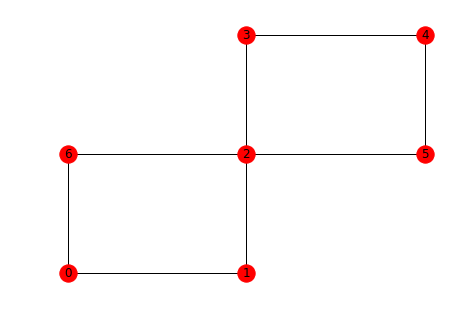
\includegraphics[width=.28\textwidth]{1-0}
}
\qquad
\subfloat[Concorde=8]{
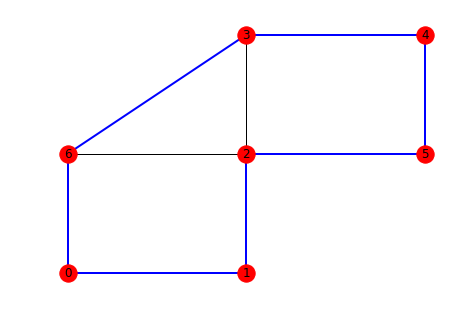
\includegraphics[width=.28\textwidth]{1-1}
}
\qquad
\subfloat[K-IMPROV=8, K=2]{
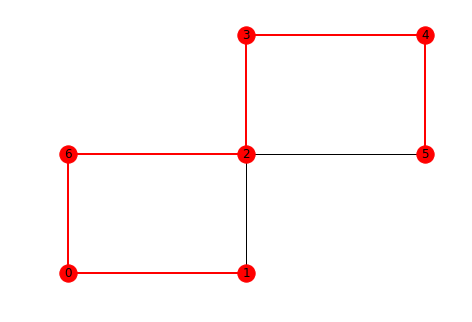
\includegraphics[width=.28\textwidth]{1-2}
}
\caption{}
\end{figure}

\begin{figure}[H]
\centering
\subfloat[n=8, m=8]{
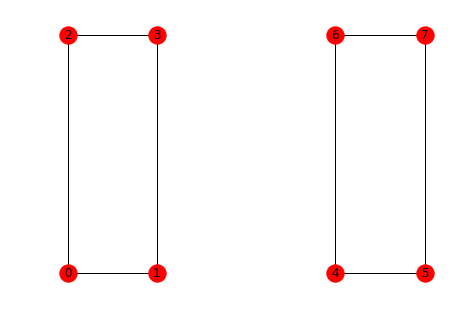
\includegraphics[width=.28\textwidth]{2-0}
}
\qquad
\subfloat[Concorde=10]{
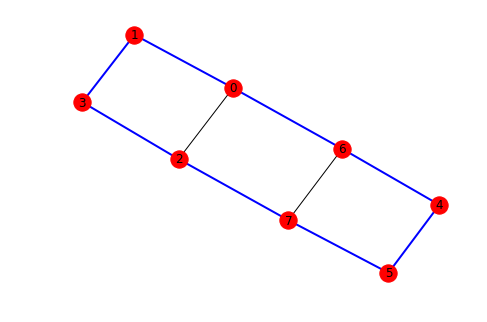
\includegraphics[width=.28\textwidth]{2-1}
}
\qquad
\subfloat[K-IMPROV=10, K=1]{
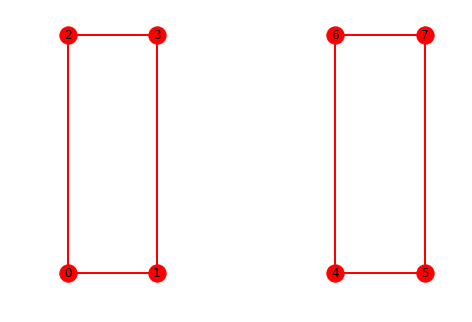
\includegraphics[width=.28\textwidth]{2-2}
}
\caption{}
\end{figure}

\subsubsection{Генерация случайных тестов}
Алгоритм тестировался на случайном графе модели Эрдеша-Реньи $G(n, m)$ с разными значениями $n$ и $m$. Также возможно тестирование на графе модели $G(n, p)$ с разными значениями $n$ и $p$.

\inputminted{python}{erdos-renyi.py}

Поскольку в расширенной версии статьи утверждение доказано для $K=15$, запуски проводились именно при таком значении $K$.

\begin{figure}[H]
\centering
\subfloat[n=10, m=20]{
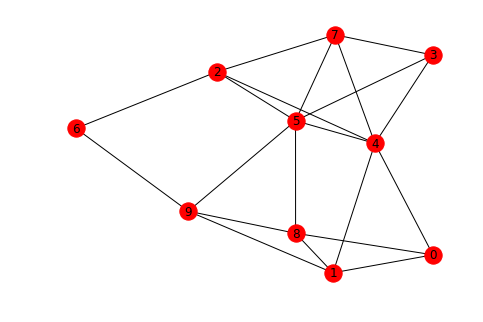
\includegraphics[width=.28\textwidth]{3-0}
}
\qquad
\subfloat[Concorde=10]{
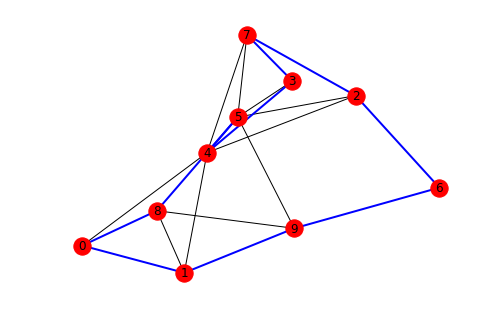
\includegraphics[width=.28\textwidth]{3-1}
}
\qquad
\subfloat[K-IMPROV=10, K=3]{
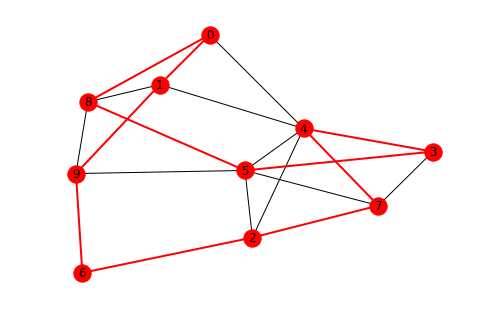
\includegraphics[width=.28\textwidth]{3-2}
}
\caption{}
\end{figure}

\begin{figure}
\centering
\subfloat[n=20, m=180]{
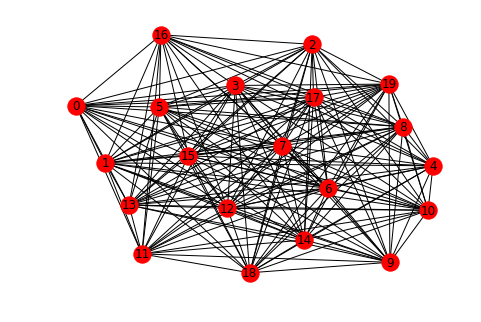
\includegraphics[width=.28\textwidth]{4-0}
}
\qquad
\subfloat[Concorde=20]{
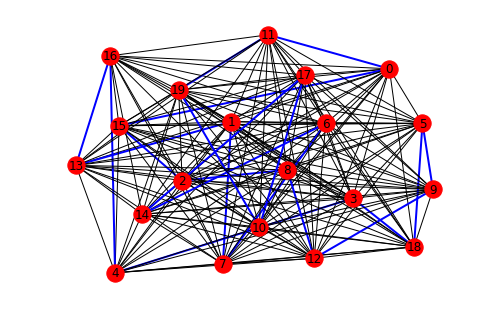
\includegraphics[width=.28\textwidth]{4-1}
}
\qquad
\subfloat[K-IMPROV=22, K=3]{
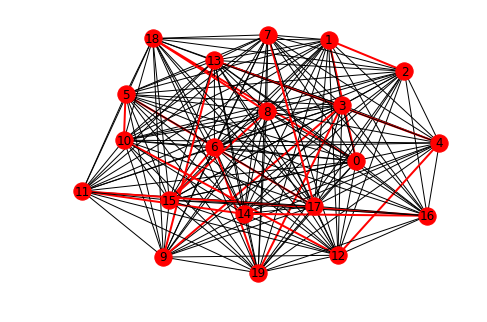
\includegraphics[width=.28\textwidth]{4-2}
}
\caption{}
\end{figure}

Расчёты показывают, что алгоритм (даже в своей оптимальной реализации) очень неэффективен при $n>20$ (см. Таблицу \ref{esttimetable}). Поэтому применялся следующий подход: считалось точное значение при помощи Concorde, запускался алгоритм и  останавливался, как только давал достаточное приближение. Это позволило провести очень много тестов. В частности, можно было проверить, какое значение $K$ необходимо, чтобы достичь нужного приближения на случайном графе $G(n, m)$, и для каких параметров $n$ и $m$ это $K$ максимально.

\begin{center}
\begin{tabular}{|l|l|l|}
\hline
$n$ & Число итераций на 1 шаг & Оценочное время работы, мин \\ \hline
17 & 131036 & 1\\ \hline
18 & 261953 & 2\\ \hline
19 & 523108 & 5\\ \hline
20 & 1042359 & 11\\ \hline
21 & 2069234 & 22\\ \hline
22 & 4084225 & 45\\ \hline
23 & 7997928 & 88\\ \hline
24 & 15505565 & 172\\ \hline
25 & 29703650 & 330\\ \hline
26 & 56138565 & 623\\ \hline
\end{tabular}
\captionof{table}{Ожидаемое время работы} \label{esttimetable}
\end{center}

\begin{figure}
\centering
\subfloat[Распределение K]{
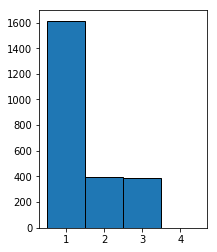
\includegraphics[height=.3\textwidth]{1}
}
\qquad
\subfloat[Распределение $n$ при $K \ge 3$]{
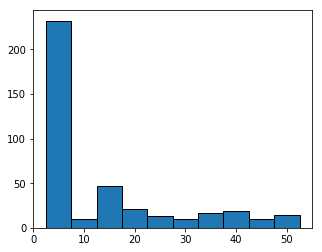
\includegraphics[width=.4\textwidth]{2}
}
\qquad
\subfloat[Распределение $m$ при $K \ge 3$]{
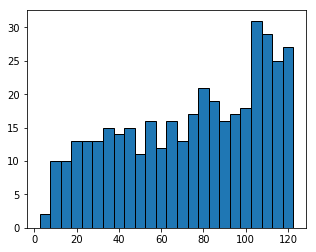
\includegraphics[width=.4\textwidth]{3}
}
\qquad
\subfloat[Распределение $\frac{m}{n}$ при $K \ge 3$]{
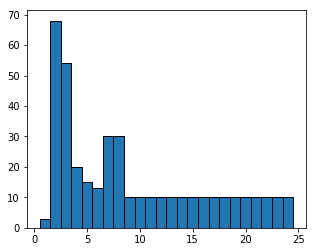
\includegraphics[width=.4\textwidth]{4}
}
\caption{}
\end{figure}

Изучение гистограмм говорит, что на графах, которые рассматривались ($n=5..50$ и $m=5..120$ с шагом 5, для каждой пары параметров генерировали и смотрели случайный граф 10 раз), наиболее часто большие $K$ требовалось при $n = \frac{m}{2} = 5$. Если не рассматривать такие маленькие графы, то в целом при $n=\frac{m}{2}$ значения были высокими, равно как они становились высокими при приближении графа к полному. Так или иначе, на рассматриваемых графах для достижения нужного приближения не потребовалось $K > 4$ (хотя если бы мы не останавливали алгоритм, он дал бы более точное приближение, использовав при этом б\'{о}льшие значения $K$).

\section{Выводы}
Алгоритм продемонстрировал свою работоспособность, но при этом очень большая константа не позволяет применять его на практике (алгоритм точного решения задачи TSP перебором с отсечениями Concorde был в сотни раз быстрее). Более того, наш алгоритм решает очень специфическую задачу, $(1, 2)-TSP$, которая вряд ли встречается в реальной жизни.
\bibliography{bibliography}
\end{document}
